\documentclass{article}
\usepackage{hyperref}
\usepackage{amsmath}
\usepackage{graphicx}
\begin{document}
\section*{Problem 2}
\subsection*{a.}
\
We used a DCGAN implementation from \href{https://pytorch.org/tutorials/beginner/dcgan_faces_tutorial.html}{PyTorch}.
They used the celeba dataset to train their DCGAN
and it was trained with these following hyperparameters:
\begin{center}
\begin{tabular}{|c|c|}
\hline
& Params for DCGAN Paper \\ \hline
Resolution & 64x64x3 \\ \hline
Latent Space Dim & 100 \\ \hline
Epochs & 5 \\ \hline
Learning Rate & 0.0002 \\ \hline
Beta1 (Adam) & 0.5 \\ \hline
\end{tabular}
\end{center}

The \href{https://arxiv.org/pdf/1511.06434.pdf}{paper for DCGAN} suggested the
hyperparameters of learning rate = 0.0002 and $beta_1=0.5$ so
the only hyperparameter that was changed from the source code was the number of epochs.
This depended on how many datapoints (images) were in the dataset. The celeba dataset
has about 200k images so 5 epochs were sufficient for them. Our dataset had
TODO and thus the following hyperparameters:
\begin{center}
\begin{tabular}{|c|c|}
\hline
& Params for our DCGAN \\ \hline
Resolution & 64x64x3 \\ \hline
Latent Space Dim & 100 \\ \hline
Epochs & TODO \\ \hline
Learning Rate & 0.0002 \\ \hline
Beta1 (Adam) & 0.5 \\ \hline
\end{tabular}
\end{center}

\subsubsection*{Issue 1 - Resolution:}
I tried changing the dimensions of the data to a higher resolution but I couldn't resolve some error that popped up relating
to the dimensions of some vector and I wasn't able to fix it. So I decided to
keep the resolution at 64x64.

\subsubsection*{Issue 2 - Seeding:}
Heres the order of operations:
$$
\text{Seeding}
\rightarrow
\text{Training dataset augmentation and creation}
\rightarrow
\text{Fixed noise}
\rightarrow \dots
$$

\noindent This fixed noise was used to keep track of how the legos turned
out over time and since the dataset batching and augmentation happened before
the fixed noise, when trying to load the trained model, the fixed noise would look
different without the training dataset. The easy fix would be to change the order
at which it happens:
$$
\text{Seeding}
\rightarrow
\text{Fixed noise}
\rightarrow
\text{Training dataset augmentation and creation}
\rightarrow \dots
$$

\subsection*{b.}
TODO

\subsection*{c.}
TODO
\begin{center}
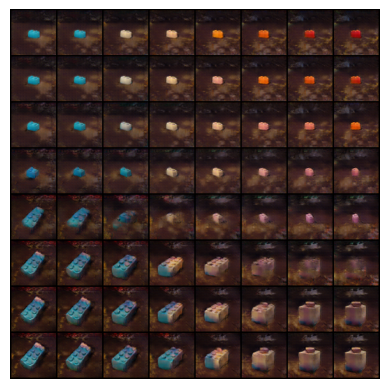
\includegraphics[scale=1]{seed_69,0,23,42,62_interpolation}
\end{center}

\newpage
\subsubsection*{Issue 3 - Lego Inconsistency:}
Interpolating between these 4 legos:
\begin{center}
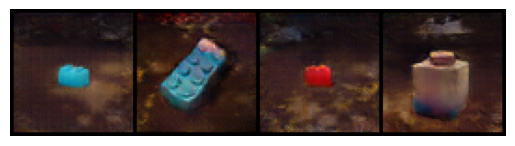
\includegraphics[scale=0.75]{seed_69,0,23,42,62_legos}
\end{center}

\noindent The interpolation gave us legos that weren't the same as the input ones
(see the bottom right is green tipped instead of pink tipped):
\begin{center}
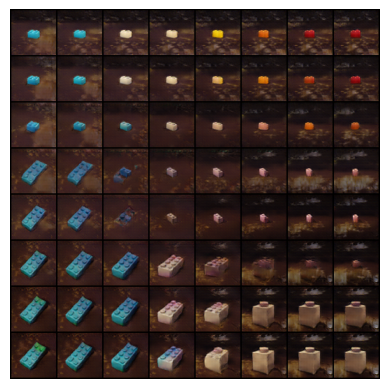
\includegraphics[scale=1]{seed_69,0,23,42,62_wrong}
\end{center}

The network takes a $B$ (batch) sized of vector of latents and
converts it to batch of images
$$
(B \times d_z \times 1 \times 1)
\rightarrow_{G}
(B \times 3 \times 64 \times 64)
$$
The fix was to individually send each image through the network and combine the images
afterwards: 
$$
(1 \times d_z \times 1 \times 1)
\rightarrow_{G}
(1 \times 3 \times 64 \times 64)
$$

\end{document}